%% ============================================================
%%  Figura: composicion del framework.
%%  Se compila POR SEPARADO y se incluye como PDF con \includegraphics,
%%  porque main.tex no se toca (regla de aislamiento de CLAUDE.md) y cargar
%%  TikZ exigiria modificar su preambulo.
%%
%%  Regenerar con:  pdflatex -interaction=nonstopmode framework_pipeline.tex
%% ============================================================
\documentclass[border=2pt]{standalone}
\usepackage[T1]{fontenc}
\usepackage[utf8]{inputenc}
\usepackage{times}
\usepackage{amsmath,amssymb}
\usepackage{tikz}
\usetikzlibrary{arrows.meta, positioning, calc}

\definecolor{bordeCaja}{gray}{0.35}
\definecolor{fondoCaja}{gray}{0.95}

\begin{document}
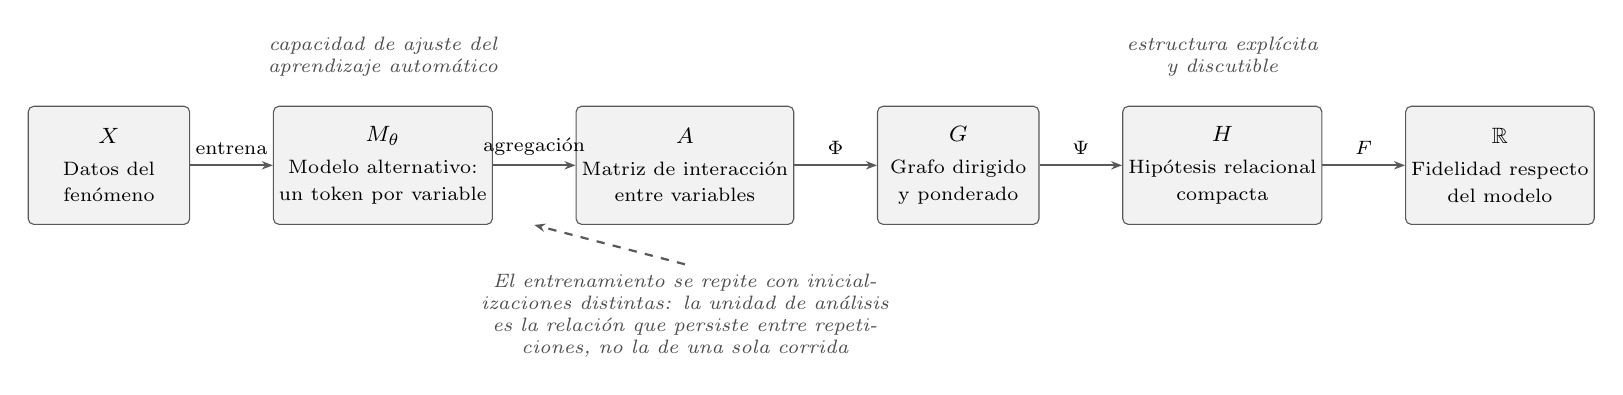
\begin{tikzpicture}[
  font=\footnotesize,
  caja/.style={draw=bordeCaja, fill=fondoCaja, rounded corners=2pt,
               minimum width=2.05cm, minimum height=1.5cm,
               align=center, inner sep=2pt},
  flecha/.style={-{Stealth[length=4pt]}, draw=bordeCaja, thick},
  etiqueta/.style={midway, above=0pt, font=\scriptsize},
  nota/.style={font=\scriptsize\itshape, align=center, text=black!70}
]

\node[caja] (x)  {$X$\\[2pt]\scriptsize Datos del\\ \scriptsize fenómeno};
\node[caja, right=1.05cm of x] (m) {$M_\theta$\\[2pt]\scriptsize Modelo alternativo:\\ \scriptsize un token por variable};
\node[caja, right=1.05cm of m] (a) {$A$\\[2pt]\scriptsize Matriz de interacción\\ \scriptsize entre variables};
\node[caja, right=1.05cm of a] (g) {$G$\\[2pt]\scriptsize Grafo dirigido\\ \scriptsize y ponderado};
\node[caja, right=1.05cm of g] (h) {$H$\\[2pt]\scriptsize Hipótesis relacional\\ \scriptsize compacta};
\node[caja, right=1.05cm of h] (r) {$\mathbb{R}$\\[2pt]\scriptsize Fidelidad respecto\\ \scriptsize del modelo};

\draw[flecha] (x) -- node[etiqueta]{entrena} (m);
\draw[flecha] (m) -- node[etiqueta]{agregación} (a);
\draw[flecha] (a) -- node[etiqueta]{$\Phi$} (g);
\draw[flecha] (g) -- node[etiqueta]{$\Psi$} (h);
\draw[flecha] (h) -- node[etiqueta]{$F$} (r);

% El consenso entre repeticiones condiciona el paso del modelo a la matriz.
\node[nota, below=0.5cm of a.south, anchor=north, text width=8.4cm] (rep)
  {El entrenamiento se repite con inicializaciones distintas: la unidad de análisis\\
   es la relación que persiste entre repeticiones, no la de una sola corrida};
\draw[flecha, dashed] (rep.north) -- ($(m.south east)!0.5!(a.south west)$);

% Que aporta cada extremo de la composicion.
\node[nota, above=0.25cm of m.north, anchor=south, text width=3.5cm]
  {capacidad de ajuste del\\ aprendizaje automático};
\node[nota, above=0.25cm of h.north, anchor=south, text width=3.5cm]
  {estructura explícita\\ y discutible};

\end{tikzpicture}
\end{document}
